 \section{Entity-Property-Quality ODP}\begin{description}
\item [CLASSIFICATION:] Good Practice.

\item [MOTIVATION:] Qualities (modifiers) are refining entities, thus refine or modify the description of another (independent) entity. They are very important in many domains. They should not be confused with selectors (e.g. left hand), although both modifiers and selectors are refining entities.

\item [AIM:] To model qualities of independent entities (e.g. position, colour, ...).

\item [STRUCTURE:] See Figure \ref{odp:EntityPropertyQuality_abstract}.
\begin{figure}[]\centering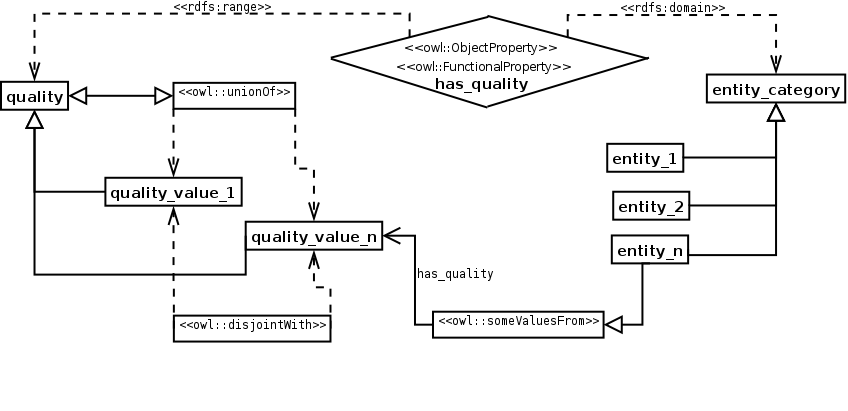
\includegraphics[width=\textwidth]{Catalogue/EntityPropertyQuality_abstract}\caption{\label{odp:EntityPropertyQuality_abstract} Abstract structure of the Entity-Property-Quality ODP.}\end{figure}

\item [SAMPLE:] See Figure \ref{odp:EntityPropertyQuality_instance}.
\begin{figure}[]\centering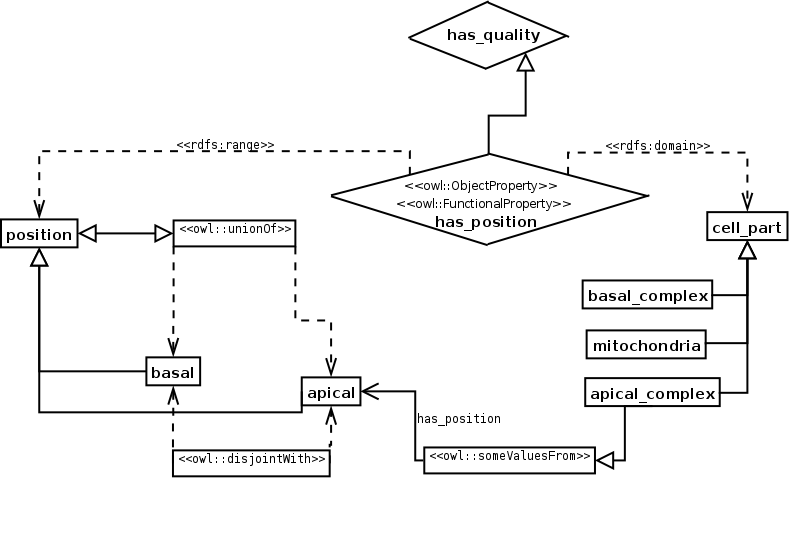
\includegraphics[width=\textwidth]{Catalogue/EntityPropertyQuality_instance}\caption{\label{odp:EntityPropertyQuality_instance} Sample structure of the Entity-Property-Quality ODP.}\end{figure}

\item [ELEMENTS:] The core of this ODP is formed by the qualities, placed in a single hierarchy (the qualities are disjoint and the superclass is covered by them, like in the Value Partition ODP). Entities are linked to qualities by a functional object property whose domain and range are the entities and the qualities, respectively.

\item [IMPLEMENTATION:] The first step is to create the qualities hierarchy, in the same way as the Value Partition ODP. Create the functional object property to link entities to qualities, adding the entities as domain and quality as range. Link entities to qualities by existential restrictions.

\item [RESULT:] The qualities that modify independent entities are modelled, and which qualities apply to which entities is defined.

\item [SIDE EFFECTS:] Proliferation of object properties (one for each quality). This ODP Cannot handle multi-aspect qualities (features).

\item [ADDITIONAL INFORMATION:] See also Entity-Feature-Value ODP and Entity-Quality ODP.

\item [REFERENCES: ] ~\begin{itemize}
\item Alan Rector (Personal Communication).
\item Mikel Egana, Alan Rector, Robert Stevens and Erick Antezana. Applying Ontology Design Patterns in bio-ontologies. EKAW 2008. LNCS 5268, pp. 7-16, 2008.\end{itemize}
\item [URL: ] \url{http://www.gong.manchester.ac.uk/odp/owl/Good_Practice_ODP/Entity_Property_Quality.owl} \end{description}